% !Mode:: "TeX:UTF-8"
\chapter{帧内无损编码优化算法}
\label{cha:c3}
本章从帧内无损编码的可优化方向的分析开始,引出本研究课题中提出的 3 个优化算法:。并且在具体描述所提出算法之前均先详细地分析了标准规定或 HM 参考软件中的实现方案,以与所提算法形成对比。

\section{帧内无损编码的可优化方向}

\section{帧内预测过程分析}
\label{cha:IntraPredDetail}
\begin{figure}
    \centering
    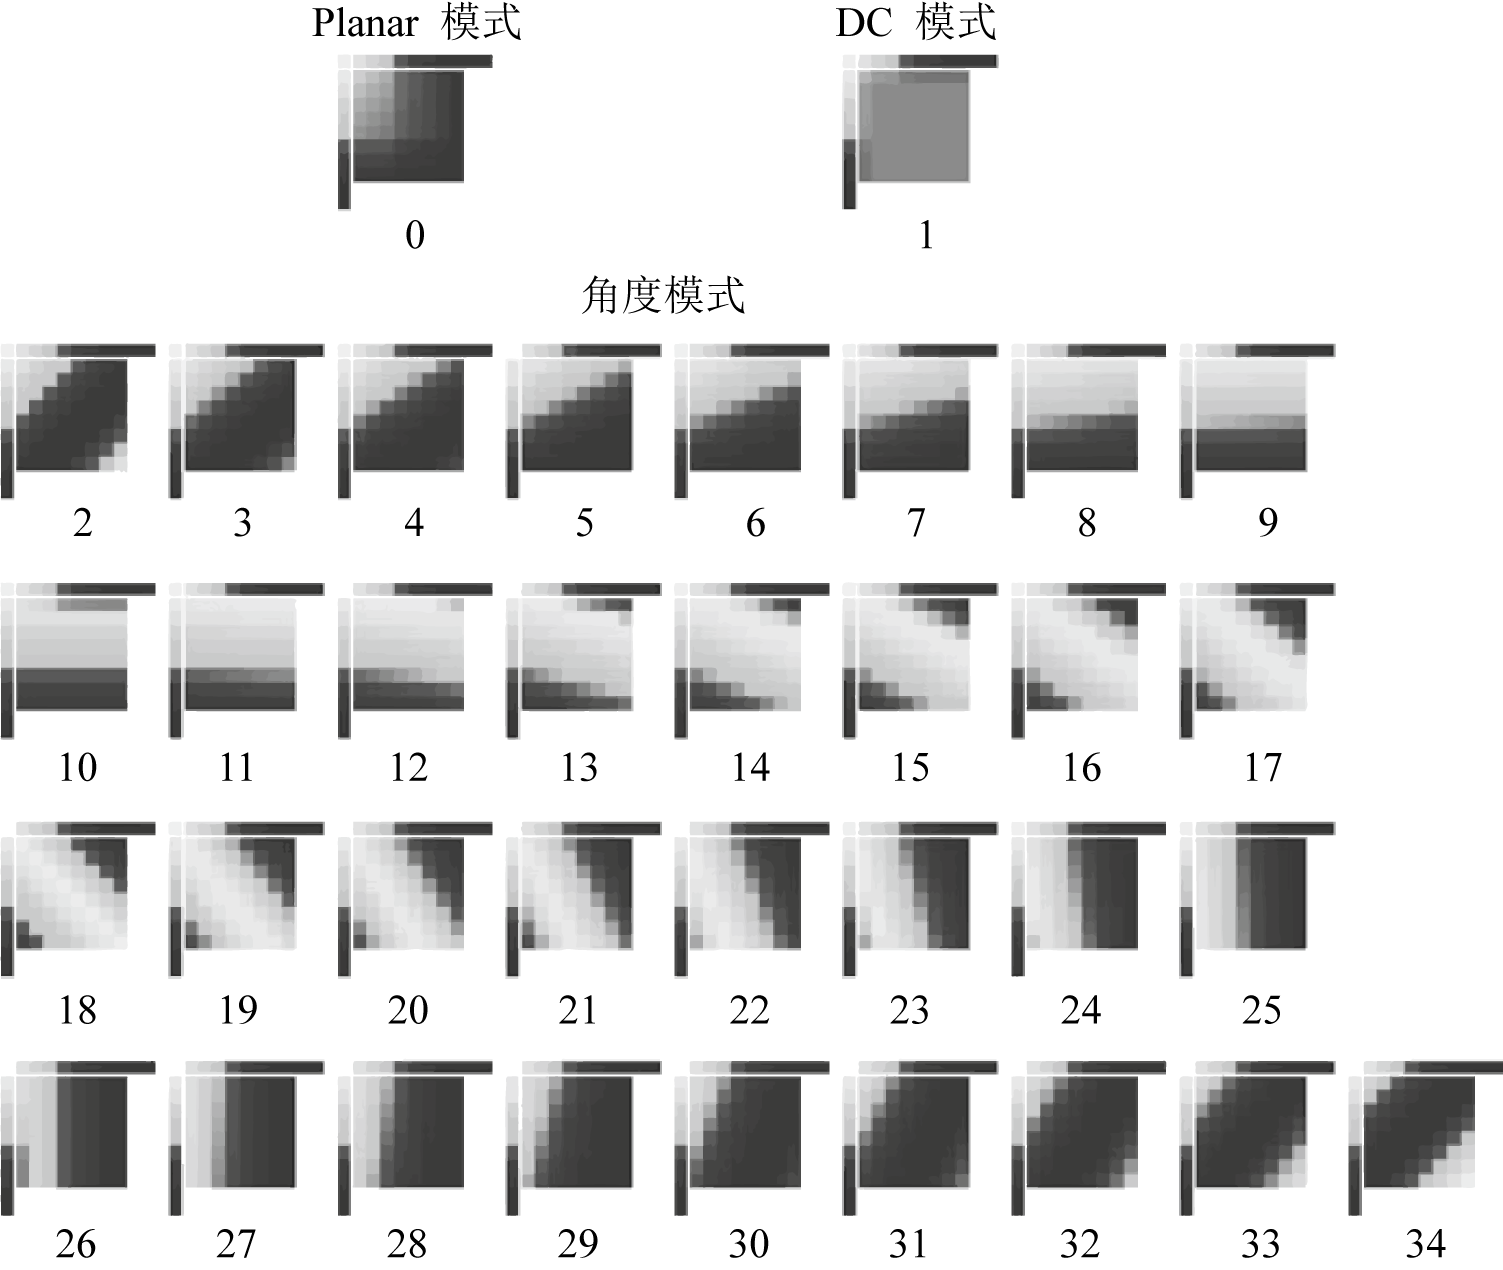
\includegraphics{IntraProjection.png}
\end{figure}

\section{帧内无损编码的预测过程优化}

\section{帧内分块决策过程分析}

\section{帧内无损编码的分块过程优化}

\section{系数编码过程分析}

\section{待编码系数的再处理}

\section{帧内无损编码优化算法性能测试}